\documentclass{article}
\usepackage[margin=1in]{geometry}
\usepackage{stmaryrd}
\usepackage{amssymb}
\usepackage{tikz}
\usepackage{ stmaryrd }
\usetikzlibrary{positioning}


\title{Interaction Diagram - Log In}
\author{ Steven Monson }

% no page number at bottom
\pagenumbering{gobble}

\begin{document}
\maketitle

\begin{center}

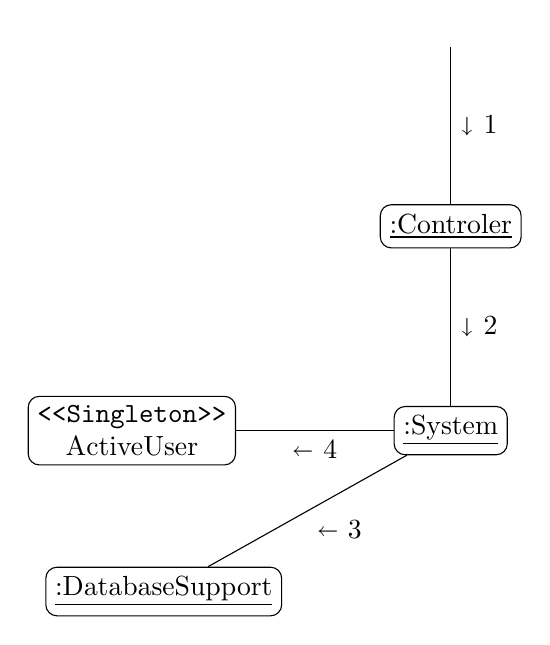
\begin{tikzpicture}[
  auto,
  block/.style = {
    rectangle,
    draw=black,
    align=center,
    rounded corners
  },
  multiple/.style = {
    rectangle, draw, rounded corners, fill= white,
    text width=9em, align= center,
    copy shadow = {
      ,fill=white, draw=black,
      shadow xshift=0.5mm, shadow yshift=-0.5mm
    }
  }
]
\node[] (start)  {};
\node[block, below=2cm of start] (cntr) {\underline{:Controler}};
\node[block, below=2cm of cntr] (system) {\underline{:System}};
\node[block, left=2cm of system] (activeUser) {\texttt{<<Singleton>>} \\ ActiveUser};
\node[block, below left=2cm of system] (db)  {\underline{:DatabaseSupport}};

\draw (start) -- (cntr) node[midway]{$\shortdownarrow$ 1};
\draw (cntr) -- (system) node[midway]{$\shortdownarrow$ 2};
\draw (system) -- (db) node[midway]{$\shortleftarrow$ 3};
\draw (system)--(activeUser) node[midway]{$\shortleftarrow$ 4};


\end{tikzpicture}

\vspace{0.5cm}

\begin{enumerate}
  \item \texttt{b:= logIn(uID:String, pw:String):boolean}
  \item \texttt{b:= logIn(uID:String, pw:String):boolean}
  \item \texttt{b:= checkCredential(uID:String, pw:String):boolean}
  \item \texttt{b:=setActiveUser(uID:String):boolean}

  
\end{enumerate}
\end{center}

\end{document}
